\documentclass{article}
\usepackage{amsmath}
\usepackage[utf8]{inputenc}
\usepackage[T1]{fontenc}
\usepackage[spanish]{babel}
\usepackage[hidelinks]{hyperref}
\usepackage{graphicx}
\usepackage{titling}
\usepackage{float}
\usepackage{longtable}
\usepackage[text={18cm,21cm},centering]{geometry}
\usepackage{hyperref} \hypersetup{ colorlinks=true, linkcolor=blue, filecolor=magenta,
urlcolor=blue, }
\usepackage{listings}
\usepackage{xcolor}
\usepackage{booktabs}

\begin{document}

\begin{titlepage}
    \centering
    {\bfseries\LARGE Universidad de La Habana \par}
    \vspace{1cm}
    {\scshape\Large Facultad de Matemática y Computación \par}
    \vspace{3cm}
    {\scshape\Huge Proyecto de Diseño de Análisis y ALgoritmos\par}
    \vfill

    {\Large Javier Rodríguez Sánchez C-411 \par}
    {\Large Juan Carlos Espinsosa Delgado C-411 \par}
    {\Large Alex Sierra Alcalá C-411 \par}

    \vfill
    {\href{https://github.com/alexsierra45/daa}{Proyecto en github} \par}
\end{titlepage}

\tableofcontents

\newpage

\section{El Laberinto}

\subsection{Ejercicio}

En tiempos antiguos, esos cuando los edificios se derrumbaban por mal tiempo y la conexión mágica era muy lenta, los héroes del reino se aventuraban en el legendario laberinto, un intrincado entramado de pasillos, cada uno custodiado por una bestia mágica. Los pasillos sólo podían caminarse en un sentido pues un viento muy fuerte no te dejaba regresar. Se decía que las criaturas del laberinto, uniendo sus fuerzas mágicas (garras y eso), habían creado ciclos dentro de este, atrapando a cualquiera que entrara a ellos en una especie de montaña rusa sin final en la que un monstruo se reía de ti cada vez que le pasabas por al lado, una locura.

El joven héroe Juan Carlos, se enfrentaba a una prueba única: desmantelar los ciclos eternos y liberar los pasillos del laberinto para que su gente pudiera cruzarlo sin caer en los bucles infinitos de burla y depravación.

Cada vez que el héroe asesinaba cruelmente (no importa porque somos los buenos) a la criatura que cuidaba una un camino, este se rompía y desaparecía. Juan Carlos era fuerte, pero no tanto, debía optimizar bien a cuántos monstruos enfrentarse. Ayude al héroe encontrando la mínima cantidad de monstruos que debe matar para eliminar todas las montañas rusas de burla y depravación.

\subsection{Abstracción}

De nuestro problema se puede crear la siguiente representación:

Tenemos un grafo $G(V,E)$ dirigido en el cual debemos encontrar la cantidad mínima de aristas a eliminar tal que el grafo resultante sea acíclico. Esto es un conocido problema NP-completo conocido en la literatura como Minimum Feedback Arc Set.

Nuestro siguiente paso será demostrar que nuestro problema es NP-completo mediante una reducción polinómica desde el problema de Minimum Vertex Cover (MVC) visto en clases, que es NP-completo. Para hacerlo, transformaremos nuestro problema en un problema de decisión, y una instancia de MVC a una instancia de nuestro problema, de tal forma que resolverlo permita resolver MVC.

Primero, demostraremos que el problema pertenece a la clase NP:

Dado un grafo y una posible solución, es fácil verificar en tiempo polinomial si el conjunto de aristas dado al ser eliminado da como resultado un grafo acíclico. Solo es necesario hacer un recorrido DFS para verificar la no existencia de aristas de retroceso, lo cual indica que se está intentando regresar a un nodo ya visitado, de donde el grafo resultante tendría al menos un ciclo.

\textbf{Definiciones:}

\begin{itemize}
    \item Se define Minimum Vertex Cover (MVC) de un grafo no dirigido $G = (V, E)$ y un número $ k $, el problema consiste en determinar si existe un subconjunto $ C \subseteq V $ de tamaño a lo sumo $ k $, tal que al menos una de las dos terminales de cada arista en $ E $ esté en $ C $.
    \item Se define Minimum Feedback Arc Set (MFAS) de un grafo dirigido $ G = (V, E) $ y un número $ k $, el problema es determinar si existe un subconjunto $ F \subseteq E $ de tamaño a lo sumo $ k $, tal que al eliminar las aristas en $ F $, el grafo resultante sea acíclico.
\end{itemize}


\subsection{Descripción de la Reducción}

Dada una instancia de Minimum Vertex Cover con:

- Un grafo $ G = (V, E) $
- Un número $ k $,

nuestro objetivo es decidir si existe un conjunto de vértices de tamaño a lo sumo $ k $ que cubra todas las aristas del grafo.

Debemos construir un grafo $ G' = (V', E') $ que sea una instancia del problema de Minimum Feedback Arc Set. En este grafo, resolver el problema MFAS será equivalente a resolver la instancia original de MVC.

\subsubsection{Construcción del Grafo $ G' $ para MFAS}

\begin{enumerate}
    \item \textbf{Partiendo de $G$:} Partimos del grafo $ G = (V, E) $ de la instancia de MVC.
    \item \textbf{Transformación a un grafo para MFAS:}
        \begin{enumerate}
            \item Para cada nodo $ u \in V $, reemplaza el nodo con 2 nuevos nodos $ u_1, u_2 $ y una arista dirigida $ e = (u_1, u_2) $ (llamémosle aristas directas a las aristas de este tipo).
            \item Para cada arista $ e = (u, v) \in E $, se reemplaza la arista $ (u, v) $ con las aristas dirigidas $ (u_2, v_1) $ y $ (v_2, u_1) $. (llamémosle aristas indirectas a las aristas de este tipo).
        \end{enumerate}
    \item \textbf{Propiedad:} Cada ciclo creado en $ G' $ corresponde a una arista en el grafo original $ G $. En particular, cada arista en $ G $ crea un ciclo de 4 vértices en $ G' $.
    \item \textbf{Propiedad:} Todos los nodos de $G'$ del tipo $x_1$ tienen outdegree 1, mientras que todos los nodos del tipo $x_2$ tienen indegree 1.
    \item \textbf{Propiedad:} En $G'$ no hay aristas entre nodos del tipo $x_1$ y tampoco entre nodos del tipo $x_2$.
    \item \textbf{Observación:} Dada una solución factible de Minimum Feedback Arc Set donde se hayan usado aristas indirectas se puede obtener una solución usando solo aristas directas:

    Demostración: Sea $C$ el conjunto de aristas de la solución factible, sea $(v_2, u_1)$ una arista indirecta que pertenece a $C$. Pero por construcción, $outdegree(v_2) = indegree(u_1) = 1$, de donde podemos inferir que si $(v_2, u_1)$ pertenece a algún ciclo, entonces $(v_1, v_2)$ y $(u_1, u_2)$ también pertencen. Por tanto se puede eliminar a $(v_2, u_1)$ de $C$ y añadir a $(v_1, v_2)$. Notemos que esta arista no pertenece previamente a $C$, debido a que, al ser el conjunto de ciclos que contienen a $(v_2, u_1)$ subconjunto del conjunto de ciclos que contienen a $(v_1, v_2)$, se podría simplemente eliminar $(v_2, u_1)$ y seguiría siendo una solución factible, entrando en contradicción con la minimalidad de $C$ supuesta inicialmente. Finalmente, estamos eliminando una arista indirecta y añadiendo otra directa, siguiendo iterativamente el algoritmo descrito será posible obtener una solución usando solo aristas directas.
\end{enumerate}

\subsection{Relación entre los Conjuntos}

Dado un grafo no dirigido $ G = (V, E) $, un conjunto $ C $ de vértices es de cobertura si y solo si el conjunto de aristas asociadas a dichos vértices es solución de la instancia de Minimum Feedback Arc Set correspondiente a dicho grafo $ G $.

\subsubsection{Demostración}

\begin{enumerate} 
    \item \textbf{Vertex Cover a Minimum Feedback Arc Set:}
        \begin{enumerate}
            \item Si en el grafo original $ G $, un vértice $ u \in C $ está en el conjunto de vértices de cobertura, entonces en $ G' $, eliminaremos la arista $ (u_1, u_2) $, eliminando todos los ciclos en los que esta está presente.
            \item Supongamos que luego de eliminar las aristas mencionadas anteriormente (las que representan a los vértices de la cobertura), queda algún ciclo creado en la construcción de $ G' $. Como este ciclo representa una arista en $ G $, podemos decir que esta no estaba cubierta por ninguno de los vértices del conjunto de cobertura mínima. Contradicción.
            \item Supongamos que existe un ciclo $(x_{1,1}, x_{2, 1}, x_{1, 2}, x_{2, 2}, \dots, x_{1, 1})$ en $G'$ distinto a los asociados a aristas de $G$. Tomemos una secuencia cualquiera de 4 nodos $S = (x_{1, j}, x_{2, j}, x_{1, j + 1}, x_{2, j + 1})$ y veamos que existe la arista indirecta $(x_{2, j}, x_{1, j + 1})$, de donde entre los nodos $x_j, x_{j + 1}$ existe una arista en $G$, además en $G'$ no han sido eliminadas ni $(x_{1, j}, x_{2, j})$ ni $(x_{1, j + 1}, x_{2, j + 1})$. De esto podemos inferir que $S$ contiene al menos un ciclo de los asociados con aristas de $G$, las cuales no estarían cubiertas. Contradicción.         
        \end{enumerate}
        Luego de la eliminación de las aristas correspondientes en $ G' $ al conjunto de vértices de cobertura mínima de $ G $ no deja ciclos en $ G' $, por tanto $|MVC(G)| \geq |MFAS(G')|$.
    \item \textbf{Minimum Feedback Arc Set a Vertex Cover:}
        \begin{enumerate}
            \item Eliminar un ciclo de los que se crearon en la construcción de $ G' $ es equivalente a cubrir una arista en $ G $, ya que eliminar una arista directa presente en dicho ciclo representa seleccionar un vértice que cubre la arista original en $ G $.
            \item Si eliminamos un conjunto de aristas de $ G' $ de manera que no queden ciclos  en $ G' $, esto corresponde a haber seleccionado un conjunto de vértices en $ G $ que cubren todas las aristas.
        \end{enumerate}
        Luego de seleccionar los nodos en $G$ relativos a las aristas eliminadas en $G'$, todas las aristas de $G$ quedan cubiertas, de donde $|MFAS(G')| \geq |MVC(G)|$.
\end{enumerate}

Queda claro entonces que $|MVC(G)| = |MFAS(G')|$.

\subsection{Conclusión}

Este análisis demuestra que aunque no sabemos cómo resolver nuestro problema o la cobertura de vértices de manera eficiente, si existiera una solución eficiente para \textbf{Minimum Feedback Arc Set} podríamos resolver eficientemente cualquier instancia de Minimum Vertex Cover y por tanto el MFAS es al menos tan difícil como MVC.

La transformación de $ G $ a $ G' $ se realiza en tiempo polinómico, finalmente queda demostrado que \textbf{Minimum Feedback Arc Set} es NP-completo.

\subsection{Solución Exacta}

Una solución exacta para este problema consiste en comprobar cada uno de los subconjuntos posibles de aristas, buscando el menor tamaño tal que el grafo quede acíclico luego de eliminar dichas aristas. Esta solución posee una complejidad temporal $O(2^{|E|} \cdot (V + E))$

\subsubsection{Optimización con Búsqueda Binaria}

Para optimizar la búsqueda del tamaño mínimo del conjunto de aristas a eliminar, podemos emplear una estrategia combinando fuerza bruta con búsqueda binaria. La idea es usar búsqueda binaria sobre el tamaño del conjunto de aristas a eliminar.

Este enfoque permite reducir significativamente el espacio de búsqueda al enfocarse en tamaños específicos y verificar su viabilidad mediante un algoritmo adaptado.

\section{Tramposo}

\subsection{Ejercicio}

Javier está pasando un curso de Diseño y Análisis de Algoritmos. Este año, por primera vez en la historia, los profesores han decidido evaluar el curso mediante un examen final y Javier se ha dado cuenta de que, a grandes rasgos, está frito. A pesar de ser un poco barco, es de hecho un muchacho inteligente y rápidamente se da cuenta de que su única forma de aprobar era hacer trampa. El día de la prueba, Javier se sentó en el asiento que estaba entre Hansel y Elena para fijarse, con la esperanza de que, uniendo las preguntas respondidas por cada uno, se pudiera formar un examen correcto.

El examen tiene $n$ preguntas, ordenadas en la hoja. Elena y Hansel pueden no ser capaces de responder cada uno el examen entero, pero todas las preguntas que responden están correctas. Se conoce cuáles preguntas respondió cada uno y se reciben como dos listas ordenadas de enteros entre $1$ y $n$. Javier tiene $p$ oportunidades para mirar hacia la izquierda (hoja de Hansel) o hacia la derecha (hoja de Elena) y su agilidad mental le alcanza para ver las respuestas de $k$ preguntas consecutivas (en cualquier posición) cada vez que echa una mirada a un examen.

Ayude a Javier a saber la cantidad máxima de preguntas que puede responder con su (tramposa) estrategia.

\subsection{Abstracción}

Sean los valores $a_i$ y $b_i$ con $i\ in [1,n]$ tal que:

$$
a_i =
\begin{cases}
1 & \text{si Elena tiene la respuesta de la pregunta i} \\
0 & \text{si no la tiene}\\
\end{cases}
$$

$$
b_i =
\begin{cases}
1 & \text{si Hansel tiene la respuesta de la pregunta i} \\
0 & \text{si no la tiene}\\
\end{cases}
$$

Denominemos una observación $q_{iP} \in 2^N$ al conjunto de los índices de las preguntas respondidas por la persona P desde la posición $i$ hasta la posición $i+k-1$. Diremos que una observación es hacia A si es hacia Elena y es hacia B si es hacia Hansel.

Sea S un conjunto de observaciones, entonces llamaremos costo de S a la función $c(S)=|\bigcup S|$

El problema consiste en encontrar $max$ $c(S)$ $s.a.$ $|S|=p$

\subsection{Solución Naive}

Existen $2n$ posibles observaciones y queremos exactamente $p$ de estas. Por lo que el total de casos validos seria $
\begin{pmatrix}
2n \\
p
\end{pmatrix}
$. Por cada combinación, por cada oportunidad se deben tener en cuenta los posibles $k$ problemas que contiene. Por lo que la complejidad final sería $
\begin{pmatrix}
2n \\
p
\end{pmatrix}
pk$.

Es evidente que al explorar todas las combinaciones de tamaño $p$, se obtendrá la respuesta correcta.

\subsection{Solución propuesta: Programación dinámica}

El algoritmo consiste en computar cuál es la mayor cantidad de problemas que se pueden resolver partiendo de la posición $i$ (con $1\leq i\leq n$), contando con $p_i$ (con $1\leq p_i\leq p$) oportunidades en cada uno de los posibles escenarios. Cada escenario consiste en ver cuáles de los siguientes $k-1$ ejercicios son observados desde $A$ o $B$ respectivamente a partir de la posición $i$ por una ventana que comience antes de dicha posición. En otras palabras, si durante una oportunidad se observó a partir de un valor anterior a $i$, es posible que las primeras posiciones del intervalo sean observadas por un intervalo anterior. Por lo que se analizan para $k_A$ y $k_B$ $(0\leq k_A,k_B\leq k)$ posibles siguientes posiciones vistas desde una ventana previa.

Para un estado $(i,k_A,k_B,p_i)$ su valor depende de los estados:

\begin{enumerate}
    \item i. $(i+1,max(k_A-1,0),max(k_B-1,0),p_i)$
    \item ii. $(i+1,k-1,max(k_B-1,0),p_i-1)$
    \item iii. $(i+1,max(k_A-1,0),k-1,p_i-1)$
    \item iv. $(i+1,k-1,k-1,p_i-2)$
\end{enumerate}

Que representan (i) no tomar ninguna oportunidad que parta de $i$, (ii) tomar una oportunidad que empiece en $i$ desde $A$, (iii) tomar una oportunidad que empiece en $i$ desde $B$ y (iv) tomar las oportunidades que empiecen en $i$ tanto en $A$ como en $B$.

Además, si hay una respuesta en la posición i, es posible ver dicha respuesta. Para esto hay diferentes escenarios:

1. Si $a_i=1$ y $k_A>0$ (el ejercicio es visto desde una oportunidad previa en A)
2. Si $b_i=1$ y $k_B>0$ (el ejercicio es visto desde una oportunidad previa en B)
3. Si $a_i=1$ y se decide hacer (ii) y (iv) (se decide hacer una oportunidad que empiece en A)
4. Si $b_i=1$ y se decide hacer (iii) y (iv) (se decide hacer una oportunidad que empiece en B)

Si ocurre uno de estos escenarios la solución debe aumentar en 1. Para más formalidad sean $r_A$ y $r_B$ tal que:

$$
r_A =
\begin{cases}
1 & \text{si } k_A>0\\
0 & \text{en otro caso}\\
\end{cases}
,
r_B =
\begin{cases}
1 & \text{si } k_B>0\\
0 & \text{en otro caso}\\
\end{cases}
$$

Entonces finalmente el costo quedaría:

$$
c(i,k_A,k_B,p) =
\begin{cases}
c(\text{i})+max(r_Aa_i,r_Bb_i)\\
c(\text{ii})+max(a_i,r_Bb_i)\\
c(\text{iii})+max(r_Aa_i,b_i)\\
c(\text{iv})+max(a_i,b_i)\\
\end{cases}
$$

Nota: $c(i,k_A,k_B,p_i)=0$ si $i>n$ y $c(i,k_A,k_B,p_i)=-1$ si  $p_i<0$

La respuesta del ejercicio sería $c(0,0,0,p)$

\subsubsection{Correctitud}

Sea $S=\{q_{i_1C_1},q_{i_2C_2},\dots\}$ una solución, entonces existe una secuencia válida de valores $\widehat{S}$ conformado por ((i),(ii),(iii),(iv)) que parten de $c(0,0,0,p)$ en la cual se observa $S$ y sus valores son iguales. Diremos que $\widehat{S} \rightarrow S$ si esto ocurre.

Decimos que una solución $S$ es válida si $|S|\leq p$. Y una secuencia $\widehat{S}$ es válida si $ii(\widehat{S}) + iii(\widehat{S}) + 2 \cdot iv(\widehat{S}) \leq p$.

Si $n=1$, existen 4 posibles valores de $S$: $\{\}$, $\{q_{1A}\}$, $\{q_{1B}\}$, $\{q_{1A},q_{1B}\}$, y trivialmente a cada una se le corresponde la secuencias $\{$(i)$\}$,$\{$(ii)$\}$,$\{$(iii)$\}$, $\{$(iv)$\}$. Entonces, si $S$ es una solución válida para $p$, $\widehat{S}$ también es una secuencia válida y el costo asociado a $\widehat{S}$ es igual a $c(S)$.

Supongamos que $\exists N \forall j, \forall S=\{q_{i_1C_1}, q_{i_2C_2,\dots}\}: ((q_{jA} \in S \lor q_{jB} \in S) \implies j<N) \implies \exists \widehat{S} : \widehat{S} \rightarrow S$.

En otras palabras, existe N tal que cualquier solución S sobre N ejercicios tiene $\widehat{S}$ tal que  $\widehat{S}\rightarrow S$

Dado $S$ una solución válida de un problema con $N+1$ ejercicios, sea $S'=S-\{q_{(N+1)A}, q_{(N+1)B}\}$. Luego, $S'$ es una solución válida de un problema de tamaño $N$. Por lo que existe $\widehat{S}'$ tal que $\widehat{S}'\rightarrow S'$.

Luego trivialmente se comprueba para cada uno de los siguientes casos:

\begin{enumerate}
    \item Si $q_{(N+1)A}\not\in S$ y $q_{1B}\not\in S$ entonces $\widehat{S}=\widehat{S}'+$(i)
    \item Si $q_{(N+1)A}\in S$ y $q_{1B}\not\in S$ entonces $\widehat{S}=\widehat{S}'+$(ii)
    \item Si $q_{(N+1)A}\not\in S$ y $q_{1B}\in S$ entonces $\widehat{S}=\widehat{S}'+$(iii)
    \item Si $q_{(N+1)A}\in S$ y $q_{1B}\in S$ entonces $\widehat{S}=\widehat{S}'+$(iv)

\end{enumerate}

Luego por inducción, $\forall S=\{q_{i_1C_1}, q_{i_2C_2},...\}\exists \widehat{S}:\widehat{S}\rightarrow S$

\subsubsection{Complejidad temporal}

Por cada posible estado se realiza una cantidad constante de operaciones. Y en total hay $npk^2$ estados. Complejidad temporal: $O(npk^2)$

\subsection{Podas}

\subsubsection{Lema 1: Empezar por ejercicio con solución}

Si existe una solución óptima $S$ con $c(S) \neq 0$, entonces existe una solución óptima S' tal que
$ \forall i:q_{iA}\in S' \implies a_i=1 \land q_{iB}\in S' => b_i=1$.

\textbf{Demostración}: 
Sea $S$ una solución óptima tal que $c(S)\neq0$ que no cumpla $\forall i:q_{iA}\in S$ => $a_i=1$ $\wedge$ $q_{iB}\in S$ => $b_i=1$. Asumamos sin pérdida de generalidad que:
$q_{iA}\in S$ $\wedge$ $a_i=0$.

Si $q_{iA}=\{\}$, entonces $|\bigcup S|=|\bigcup S/q_{iA}|$

Como $c(S)\neq 0, \exists j:a_j=1 \land b_j=1$. Sin pérdida de generalidad asumamos que $b_j=1$. Luego,
$$|\bigcup S/q_{iA}|\leq|\bigcup S/q_{iA}\cup q_{jB}|=|\bigcup S'|$$

Luego, $c(S)\leq c(S')$, pero como $S$ es óptimo: $c(S)= c(S')$

Si $q_{iA}\neq\{\}$, entonces $\exists x_1, x_2...x_r$ con $r<k,$ $x_r<k$, $\forall j,h:j<h$ => $x_j<x_h$ tal que:

$q_{iA}=\{i+x_1,i+x_2,...,i+x_r\}$

Sean $j=i+x_1$ y $y_h=x_{h+1}-x_1$. Sustituyendo

$q_{iA}= \{j,j+y_1,...,j+y_{r-1}\}$

=> $q_{iA}\subseteq q_{jA}$

=> $c(S)\leq c(S')$

Con $S'=S/q_{iA}$  $\cup$ $\{q_{jA}\}$

Pero como $S$ es óptimo: $c(S)= c(S')$

Usando este razonamiento y aplicando inducción queda demostrado.


\subsubsection{Lema 2: No repetir posiciones}

Si una solución óptima $S$ contiene las observaciones $q_{iA}$ y $q_{iB}$, existe otra solución óptima que o no contiene a $q_{iA}$ o no contiene a $q_{iB}$.

\textbf{Demostración}: 

Usando el lema 1, partamos de una solución donde todas las observaciones comiencen con una pregunta respondida.

Llamemos:
$
X_i =
\begin{cases}
\{i\} & \text{si } b_i=1\\
\{\} & \text{si } b_i=0\\
\end{cases}
$

Para cierto $i$, sean $b_i=a_i=1$. Luego:
$$c(S)=|\bigcup S|=|(\bigcup (S/q_{iB}))\cup q_{iB}|$$

$$=|(\bigcup (S/q_{iB}))\cup (\bigcup_{j=i}^{i+k-1} X_j)|$$

$$=|(\bigcup (S/q_{iB}))\cup X_i \cup (\bigcup_{j=i+1}^{i+k-1} X_j)|$$

$$\leq |(\bigcup (S/q_{iB}))\cup X_i \cup (\bigcup_{j=i+1}^{i+k} X_j)|$$

$$= |(\bigcup (S/q_{iB}))\cup X_i \cup q_{(i+1)B}|$$

$$= |(\bigcup (S'))\cup X_i|$$

Donde $S'=(S/q_{iB}) \cup q_{(i+1)B}$

Como $a_i=1$ y $q_{iA} \subseteq S'$ entonces $i$ está siendo considerada en $S'$, por lo que:

$$|(\bigcup (S'))\cup X_i|=|(\bigcup (S'))|$$

Luego:$$c(S)\leq c(S')$$

Pero $S$ es óptimo, por lo que: $$c(S)= c(S')$$

Y obtenemos una solución óptima diferente.

\subsubsection{Lema 3: Evitar solapamientos}

Sea $S$ una solución tal que $\exists i< n-k,j\leq k:q_{iA} \in S$ $\land$ $q_{(i+j)A}\in S$. Luego, existe la solución $S'=S-\{q_{(i+j)A}\} + \{q_{(i+k)A}\}$ tal que $c(S')\geq c(S)$

\textbf{Demostración}: 

$c(S)=|\bigcup (S)|=|\bigcup (S-\{q_{(i+j)A}\})\cup q_{(i+j)A}|$

Como $q_{iA} \in S$ sea $Q=\{l:a_l=1$ $\wedge$ $i+j<l< k\}$. Luego obviamente $Q=q_{(i+j)A}/q_{iA}$:

$c(S)=|\bigcup (S-\{q_{(i+j)A}\})\cup Q|$

Pero $Q\subseteq q_{(i+kA)}$, por tanto

$c(S)\leq|\bigcup (S-\{q_{(i+j)A}\})\cup q_{(i+kA)}|$

$=>c(S)\leq S'$

Con $S'=S-\{q_{(i+j)A}\} \cup \{q_{(i+k)A}\}$

Nota: El lema se aplica homológamente a $B$

\subsubsection{Lema 4: Detección de soluciones inmediatas}

Si una solución óptima $S$ contiene las observaciones $q_{iA}$ y $q_{iB}$, existe otra solución óptima que o no contiene a $q_{iA}$ o no contiene a $q_{iB}$.

\textbf{Demostración}:

Sea $P=(A,B,p,k)$ una instancia del problema ($A=\{j:a_j=1\}$ y $B=\{j:b_j=1\}$). Dado una caso de la forma $(i,k_A,k_B,p_i)$ del problema. Si se cumple:
$$
    [(n-i-k_A)/k]+[(n-i-k_B)/k]\leq p
$$

Entonces:

$$c(i,k_A,k_B,p)=\sum_{j=i}^n (a_i+b_i-a_ib_i)$$

**Demostración:**

Sea $p_A=[(n-i-k_A)/k]$ y $[p_B=(n-i-k_B)/k]$

La selección $S'=\{q_{(i+k_A+kj)A}:0<j<p_A\} \cup \{q_{(i+k_B+kj)B}:0<j<p_B\}$ es una seleccion válida, ya que $p_A+p_B<p$. Luego $\forall j>k_A(k_B) \exists h:j \in q_{hA}(a_{hB}) \wedge q_{hA}(q_{hB})\in S'$. Por lo que todos los valores a partir de la posición i pertenecen a una observación.

\subsection{Lema 4: Complejidad de las podas}

Para el lema 1: Este lema evita calcular (ii) cuando $a_i=0$, (iii) cuando $b_i=0$ y $iv$ cuando $a_i=0$ o $b_i=0$. Al solo analizar aquellos casos donde hay una respuesta, sea $m=\sum (a_i + b_i - a_ib_i)$ la cantidad de ejercicios resueltos, la complejidad baja a  $O(mpk^2)$.

Para el lema 2: Con este lema, descartamos aquellas soluciones que usen (iv) por completo. La repercusión directa es que no se analizarán los casos donde $k_A=k_B$, a excepción del $k_A=k_B=0$. Por lo que la complejidad baja a $O(np(k^2-k+1))$.

Para el lema 3: Esto nos permite calcular ventanas solapadas, haciendo que no se aplique (ii) y (iv) si $k_A>0$, ni tampoco (iii) ni (iv) si $k_B>0$

Para el lema 4: Esta poda permite resolver problemas de forma sencilla cuando $k*p\rightarrow n$ y solo añade un preprocesamiento de tamaño $O(n)$.

\begin{center}
    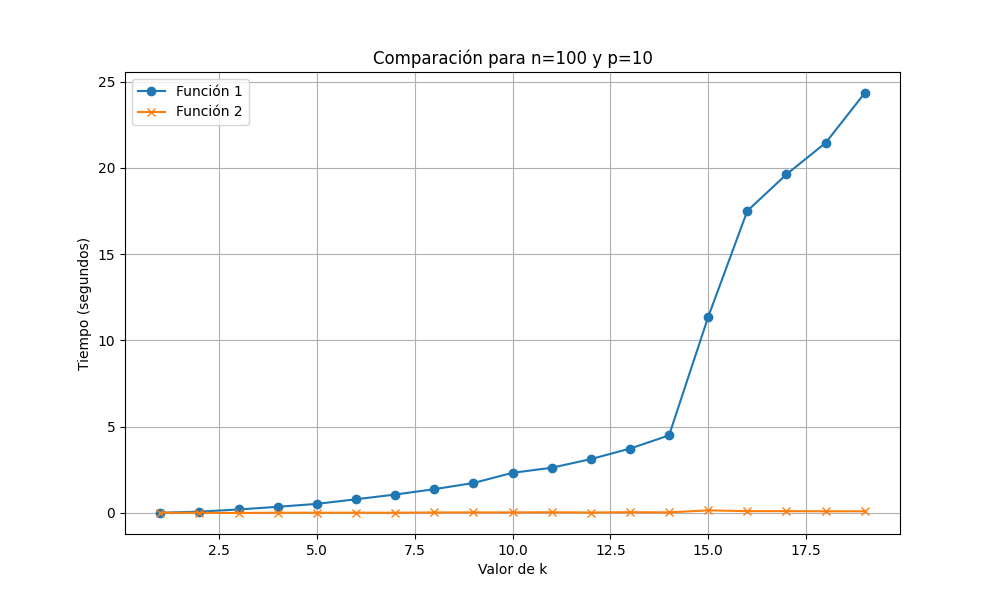
\includegraphics[height = 0.5\textheight]{problems/2/k_plot.png}
    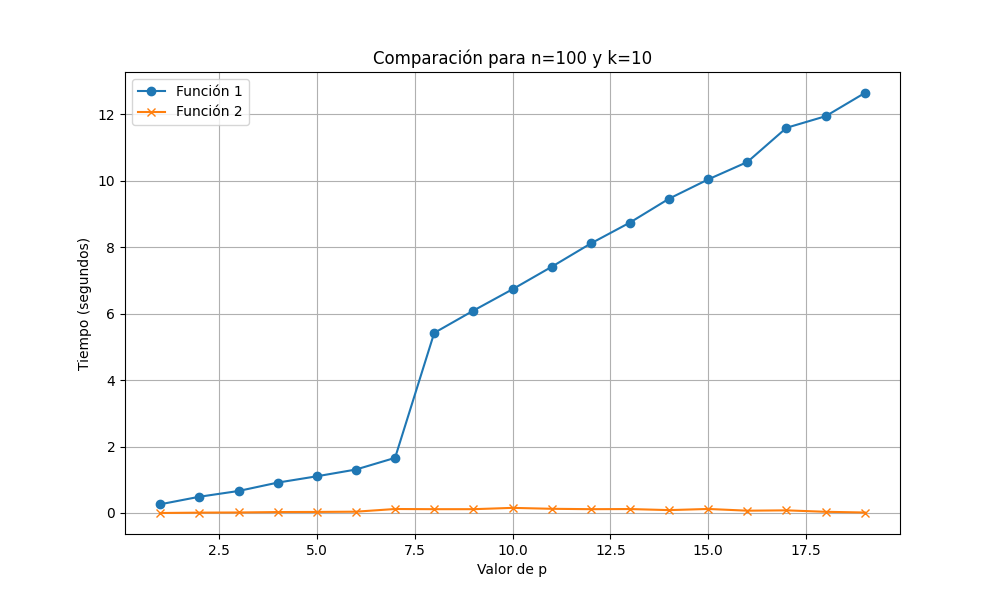
\includegraphics[height = 0.5\textheight]{problems/2/p_plot.png}
\end{center}

\section{Ciudades}

\subsection{Ejercicio}

Cuba tiene inicialmente $N$ ciudades aisladas, donde la $i$-ésima ciudad tiene una significancia de $A_i$. Alex, el Presidente de Cuba quiere conectar todas las ciudades. Él puede construir una carretera bidireccional de longitud $L$ $(L > 0)$ desde la ciudad $X$ a la ciudad $Y$ si $(A_X$ \& $A_Y$ \& $L) = L$, donde $\&$ representa el operador AND bit a bit.

¿Cuál es la longitud total mínima de las carreteras que tiene que construir para conectar todas las ciudades en Cuba? Imprime $-1$ si es imposible.

Nota: Se dice que la ciudad $X$ y la ciudad $Y$ están conectadas si existe una secuencia de ciudades $C_1, C_2, \dots, C_K$ $(K \geq 1)$ tal que $C_1 = X$, $C_K = Y$, y existe una carretera desde $C_i$ a $C_{i+1}$ $(1 \leq i < K)$. Todas las ciudades en Cuba se dicen conectadas cuando cada par de ciudades en Cuba está conectado.

\subsection{Abstracción del problema}

Sea G = (V, E) un multigrafo no dirigido tal que para cada ciudad del problema inicial tenemos un nodo en V, con un valor $A_i$ asociado al $i$-ésimo nodo. Entre los nodos $i$ y $j$ existe una arista de peso $(L > 0)$ si $(A_X$ \& $A_Y$ \& $L) = L$. Hallar el Árbol Abarcador de Costo Mínimo, a partir de ahora MST (Minimum Spanning Tree), de G.

\subsection{Observaciones}

\begin{enumerate}
    \item La ecuación $A \& x = x$, con $x > 0$ se satisface cuando $x$ es la representación de cualquier combinación de bits activos en $A$, a excepción de la combinación vacía. Escrito más formalmente, sea $f(A, i) = 1$ si el $i$-ésimo bit de $A$ esta activo, 0 en otro caso, entonces las soluciones de $A \& x$ = $x$, con $x > 0$ pertenecen al conjunto $\{x | x = \sum f(A, i) \cdot g(i) \cdot 2 ^i, g(i) \in \{0, 1\} \land \sum g(i) \geq 1\}$.
    \item Podemos considerar a G como un grafo simple y no un multigrafo ya que como el objetivo es hallar el MST de G, lo optimo siempre sera, si se va a tomar una arista de $i$ a $j$, tomar la de menos peso que sera exactamente la relativa al bit activo menos significativo de $A_i \&  A_j$, arista que evidentemente pertenece al conjunto mencionado previamente.
    \item En el árbol resultante de hallar el MST a G, para toda secuencia de nodos que forman un camino, se cumple que para cualquier par consecutivo de ellos tienen al menos un bit activo en común. Para una lista A definamos $OR(A)$ como el resultado de aplicar la operación OR bit a bit de los elementos de $A$, es decir $f(OR(A), i) = 1$ si y solo si alguno de los elementos de $A$ tiene el $i$-ésimo bit activo. De la definición y el resultado anterior se desprende que si existe una partición $A, B$ de los nodos de G, tal que $OR(A) \& OR(B)$ = 0, entonces no existiría ninguna arista entre los nodos de $A$ y $B$, por lo que no existiría el MST de G.
    
\end{enumerate}

\subsection{Solución naive}

Armar un grafo G con un nodo por cada ciudad, cada nodo $i$ con un valor asociado $A_s$. Luego pasar por cada par de nodos y construir una arista de peso igual al bit activo menos significativo entre ellos. Luego usar algún algoritmo clásico como Kruskal o Prim para hallar el MST del grafo. Para G se tiene que $|V| = O(n)$ y $|E| = O(n^2)$, de donde la complejidad de esta solución es $O(n^2 \log n)$.

\subsection{Teoría de arista liviana que cruza el corte}

\subsubsection{Definiciones}

\begin{enumerate}
    \item Un corte $(S, V-S)$ de $G=(V,E)$ no dirigido es una partición de los vértices del conjunto V.
    \item Una arista $<u,v>$ cruza el corte $(S, V-S)$ si uno de los extremos de la misma está en $S$ y el otro en $V-S$.
    \item Un corte, respeta un conjunto de aristas $A$, si no existen aristas en $A$ que crucen el corte .
    \item Una arista es liviana cruzando el corte, si tiene el menor peso entre todas las que lo cruzan .
\end{enumerate}

\subsubsection{Teorema}

\begin{enumerate}
    \item Sea $G=(V,E)$ un grafo conexo, no dirigido y ponderado.
    \item Sea $A \subseteq E$ incluido en algún MST de G.
    \item Sea $(S, V-S)$ un corte de G que respeta A.
    \item Sea $<u,v> \in E$ una arista liviana que cruza el corte $(S, V-S)$.
\end{enumerate}

Entonces, $<u,v>$ es segura para $A$. Esto significa que $A \cup \{<u, v>\} \subseteq T$, donde $T$ es un MST de G.

\subsection{Solución}

\subsubsection{Algoritmo}

Nuestro algoritmo recibe como entrada una lista $L$ de los valores asociados a cada una de las $n$ ciudades. Sea $m = max(L)$. Primeramente nuestro algoritmo instancia una variable $ans = 0$, luego por cada $0 \leq i \leq m - 1$ realizara la siguiente secuencia de pasos:

\begin{enumerate}
    \item 1) Instancia dos listas vacias $A$ y $B$.
    \item 2) Por cada elemento $v \in L$, si $f(v, i) = 1$, $A = A \cup \{v\}$, en otro caso $B = B \cup \{v\}$.
    \item 3) Si $A \ne \empty$, hacemos $ans += (|A| - 1) \cdot 2^i$ y $B = B \cup \{OR(A)\}$.
    \item 4) Actualizamos la lista de nuevos valores y hacemos $L = B$.
    
\end{enumerate}

Finalmente, si $|L| = 1$ devolvemos $ans$, en otro caso -1.

\subsubsection{Explicación}

El algoritmo en la $i$-ésima iteración selecciona todos los nodos cuyo valor tengan activo el $i$-ésimo bit y los agrega a la lista $A$, al resto los agrega a $B$. Luego usa exactamente $|A| - 1$ aristas de peso $2^i$ para conectar los nodos de $A$ con un camino que pase por todos. Una vez conectados, se considera que desde la nueva componente conexa puede salir una arista de peso $2^j$ si el $j$-ésimo bit esta activo para alguno de los valores de $A$, por tanto podríamos tomar un nuevo nodo con valor $OR(A)$ y agregarlo a la lista $B$ de nodos que no participaron en esta iteración, luego actualizamos $L$ con la nueva lista de valores para la proxima iteración. Veamos que no se arma el grafo explícitamente, sin embargo iterativamente se van sumando a la respuesta los pesos de las aristas que van siendo añadidas. Nótese que al inicio de cada iteración la lista $L$ solo contiene los valores de nodos que no están conectados entre ellos, por lo tanto añadir una arista nunca generara un ciclo.

La idea principal detrás de esta implementación es que, si entre un par de nodos existe un camino que solo use aristas de peso a lo sumo $2^i$, después de la $i$-ésima iteración dichos nodos van a quedar conectados. Probemos esto por inducción:

\begin{enumerate}
    \item \textbf{Caso Base:} Para $k = 0$. Luego de la primera iteración, todos los nodos con el primer bit activo, si hay alguno, quedan conectados por la forma en la que funciona el algoritmo.\item
    \item \textbf{Hipótesis:} Para $k = i$. Sean $x, y$ nodos entre los cuales existe al menos un camino con aristas de peso a lo sumo $2^i$, entonces luego de la $i$-ésima iteración, $x, y$ quedan conectados.\item
    \item \textbf{Tesis:} Para $k = i + 1$. Sean $x, y$ nodos entre los cuales existe al menos un camino con aristas de peso a lo sumo $2^{i + 1}$. Si todas las aristas tienen peso menor que $2^{i + 1}$, dichos nodos están conectados desde la iteración pasada del algoritmo por hipótesis de inducción. Supongamos entonces que hay exactamente una arista de peso $2^{i + 1}$ (el caso en el que hay mas de una es análogo), y sean $u, v$ los nodos adyacentes a dicha arista, sin perdida de generalidad digamos que en el recorrido de $x$ a $y$ se visita primero a $u$. Entonces $x$ esta conectado con $u$ y $L$ esta conectado con $y$ desde la iteración anterior por hipótesis de inducción debido a que todas las aristas en esos caminos son de peso a lo sumo $2^i$. Por tanto en la iteración $(i+1)$-ésimo quedan conectados $x, y$ luego de añadir al grafo la arista $<u, v>$, terminando con la demostración.

\end{enumerate}

Si luego de concluir el algoritmo, la lista de valores $L$ quedo con mas de un elemento, hay al menos dos nodos que no pudieron ser conectados con caminos que usan aristas de a lo sumo el peso máximo de alguna arista del grafo. En otras palabras, no existía camino inicialmente entre ellos, por lo que la construcción de un MST sobre G es imposible, por tanto devuelve -1.

\subsubsection{Correctitud}

Probemos ahora que el valor devuelto por el algoritmo corresponde con un MST de G:

\begin{enumerate}
    \item Como se vio anteriormente, las aristas se construyen entre nodos que estaban previamente desconectados, por tanto nunca se genera un ciclo. Ademas como la lista $L$ quedo con exactamente un elemento, y por cada elemento que se eliminaba se añadía exactamente una arista, el grafo resultante es acíclico y tiene $n -1$, de donde es un árbol abarcador.
    \item Supongamos que dicho árbol abarcador no es de costo mínimo. Eso implica que existe una arista $e$ de peso $2^p$ con $p > 0$ que no es segura en el corte $(A, V - A)$ que define, y por tanto, no es liviana. De donde existe una arista $<u, v>$ de peso $2^q$ con $u \in A \land v \in V - A$, que no esta siendo tomada en el árbol. Sin embargo en el momento en que se toma la arista $e$, y debido a que $q < p$, los nodos $u, v$ no pueden estar desconectados y por tanto no pueden estar en lados diferentes de un corte. Contradicción con lo asumido, el valor obtenido corresponde con el costo del MST de G.    
\end{enumerate}

\subsubsection{Complejidad Temporal}

Por cada bit en la representación binaria de $m$ se recorre una lista que tendrá a lo sumo $n$ elementos. Complejidad $O(n \log m)$.


\end{document}